\documentclass{beamer}

\usetheme{beunitn}

\usepackage{graphicx}

\title[Performance Evaluation of TARP]{Performance Evaluation of TARP in Unstable Wireless Environments}
\author{Damiano Salvaterra \\ Simone De Carli}

\date{}

\begin{document}

%------------------------------------------------
\begin{frame}
  \titlepage%
\end{frame}
%------------------------------------------------

\begin{frame}{TARP:\ Tree-based Any-to-Any Routing Protocol}

  \begin{columns}

    % LEFT COLUMN (text)
    \begin{column}{0.55\textwidth}
      \begin{itemize}
        \item Gradient-based routing paradigm
        \item Hybrid link cost: RSSI + ETX
          \begin{itemize}
            \item RSSI:\ Received Signal Strength Indicator
            \item ETX:\ Expected Transmission Count
          \end{itemize}
        \item Reactive parent switching
      \end{itemize}
    \end{column}

    % RIGHT COLUMN (figure)
    \begin{column}{0.52\textwidth}
      \begin{figure}
        \centering
        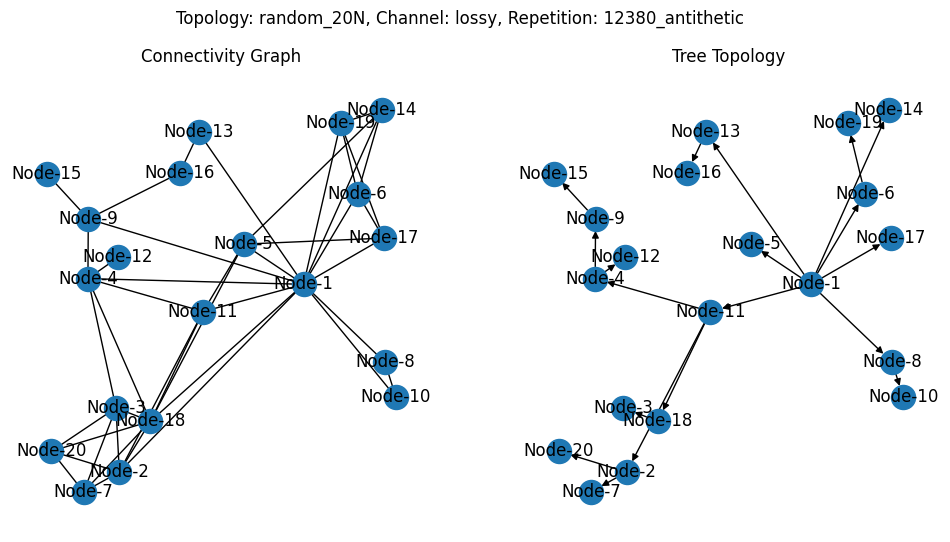
\includegraphics[trim={0 0 0 2.5cm},clip,width=\textwidth]{images/tree.png}
        \caption{\tiny Connectivity graph (left) and routing tree (right) in random topology under lossy channel conditions.}
      \end{figure}
    \end{column}

  \end{columns}

\end{frame}

%------------------------------------------------

\begin{frame}{Motivation}

  \begin{itemize}
    \item TARP was designed for WSNs in a static environment
    \item We want to evaluate its performance under realistic conditions:
      \begin{itemize}
        \item Different physical topologies (linear, grid, star, ring, random)
        \item Different channel conditions
      \end{itemize}
    \item With a tilt towards unfavorable conditions
  \end{itemize}
\end{frame}

%------------------------------------------------

\begin{frame}{Simulation Architecture: Custom DES}
  \begin{itemize}
    \item Python-based discrete event simulator
    \item Single-threaded scheduler (parallelized runs)
    \item Modular architecture:
      \begin{itemize}
        \item Node module (static, dynamic)
        \item PHY module (channel modeling)
        \item MAC module (IEEE 802.15.4)
        \item Routing module (TARP implementation)
        \item Attachable monitors for debugging and data collection
      \end{itemize}
    \item High-fidelity PHY + IEEE 802.15.4 MAC
  \end{itemize}
\end{frame}

%------------------------------------------------

\begin{frame}{Physical Layer Modeling}
  \begin{itemize}
    \item Log-distance path loss
    \item Correlated shadowing (Gudmundson model)
    \item Nakagami-$m$ fading
    \item SINR-based packet decoding
  \end{itemize}

  \vspace{0.5cm}
  \centering
  % Placeholder for channel
  \fbox{\parbox[c][3cm][c]{6cm}{\centering Here it would possibly be nice to have a visualization of something. The correlated shadowing feels like a good candidate.
  }}
\end{frame}

%------------------------------------------------

\begin{frame}{MAC and Interference Modeling}
  \begin{itemize}
    \item IEEE 802.15.4 Unslotted CSMA/CA
    \item Backoff + Retransmissions
    \item Capture Effect
    \item CCA via energy detection
  \end{itemize}
\end{frame}

%------------------------------------------------

\begin{frame}{Experimental Design}
  \begin{itemize}
    \item 5 Topologies
      \\{\small [Linear, Grid, Star, Ring, Random]}
    \item 6 Channel Profiles
      \\{\small [Ideal, Stable, Stable (Mid PL), Stable (High PL), Lossy, Unstable]}
    \item Poisson Traffic Model ($\frac{1}{\lambda} = 60s$)
    \item 50 ARV pairs (100 runs per configuration)
  \end{itemize}

  \begin{figure}
    \centering
    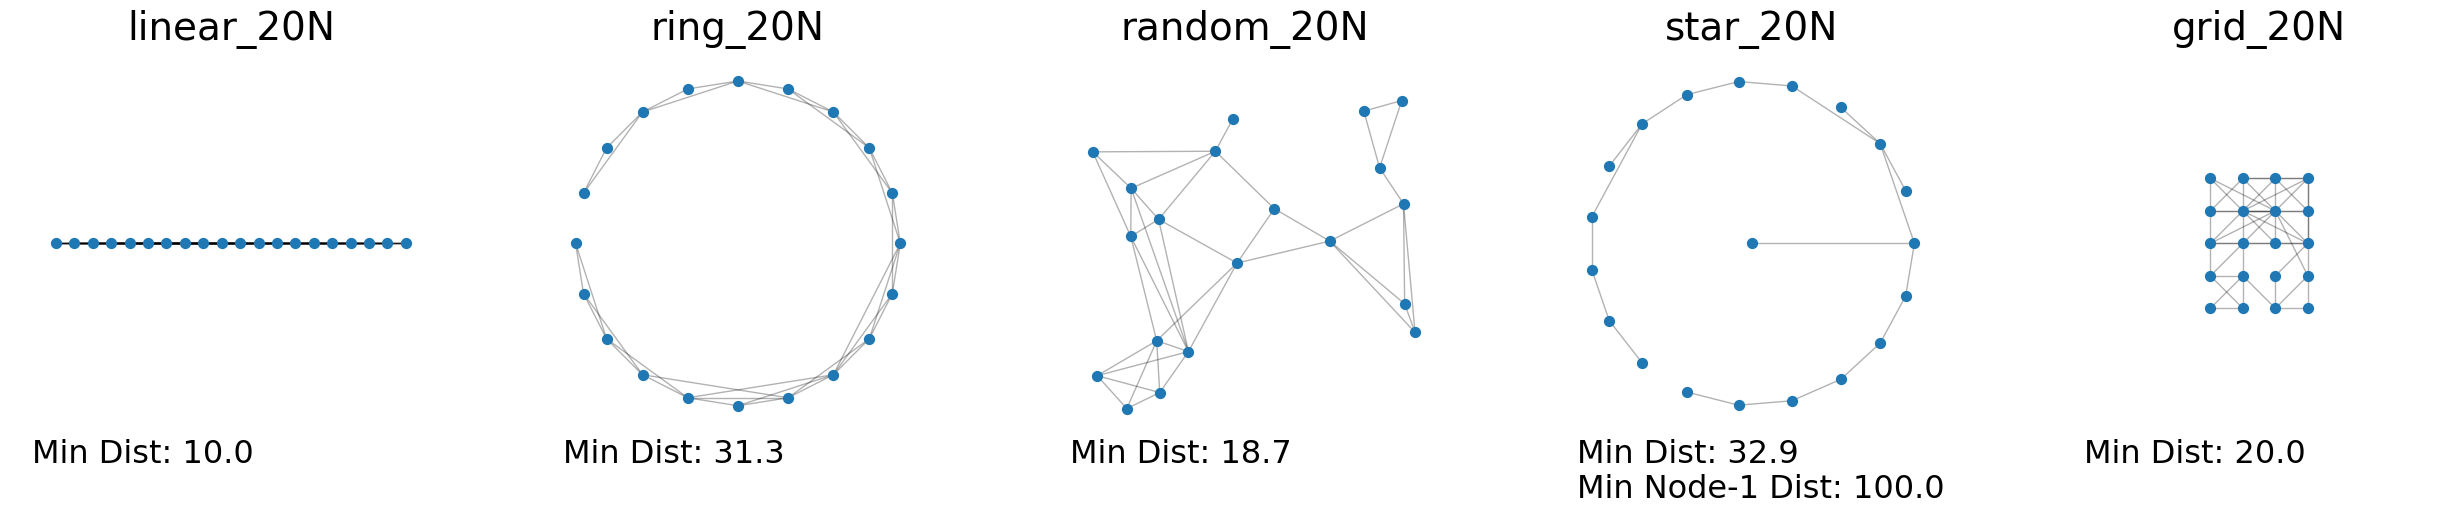
\includegraphics[width=1.05\textwidth]{images/topologies.png}
    \caption{\tiny The 5 topologies considered in the evaluation}
  \end{figure}
\end{frame}

%------------------------------------------------

\begin{frame}{Statistical Methodology}
  \begin{itemize}
    \item Independent random streams (Philox PRNG)
      {\tiny \texttt{random\_manager.get\_stream(key = "NARROWBAND\_CHANNEL/SHADOWING")}}
    \item Antithetic Random Variates (ARV)
      \begin{itemize}
        \item $F^{-1}(U)$ and $F^{-1}(1-U)$
        \item Uniform, Normal, Exponential and Nakagami-$m$ have a closed-form inverse CDF
      \end{itemize}
    \item Common Random Numbers (CRN) across configurations
    \item Bootstrap 95\% Confidence Intervals
  \end{itemize}
\end{frame}

%------------------------------------------------

\begin{frame}{Control Variates}

  Interarrival time as a control variate.

  \begin{columns}
    \begin{column}{0.5\textwidth}
      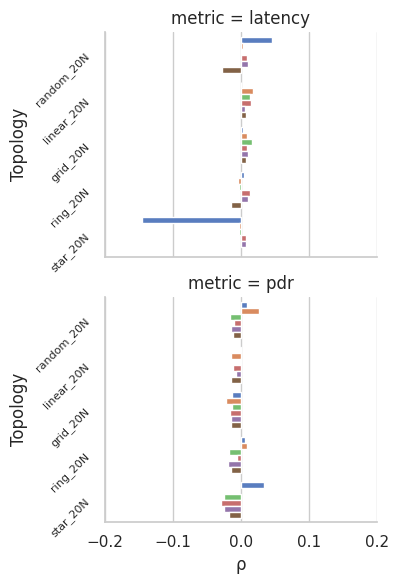
\includegraphics[width=0.85\textwidth]{images/corr_bars.png}
    \end{column}

    \begin{column}{0.5\textwidth}
      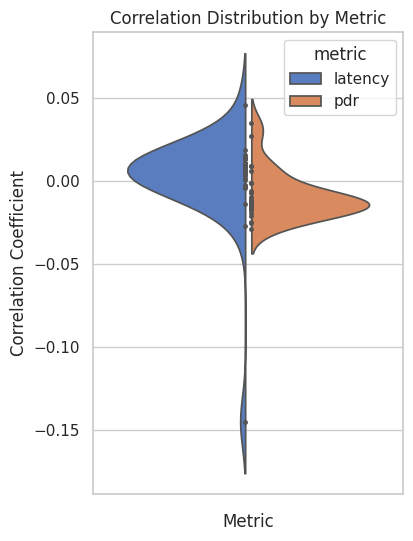
\includegraphics[width=0.9\textwidth]{images/corr_violin.png}
    \end{column}

  \end{columns}

\end{frame}

%------------------------------------------------

\begin{frame}{Results: Packet Delivery Ratio (PDR)}
  \centering
  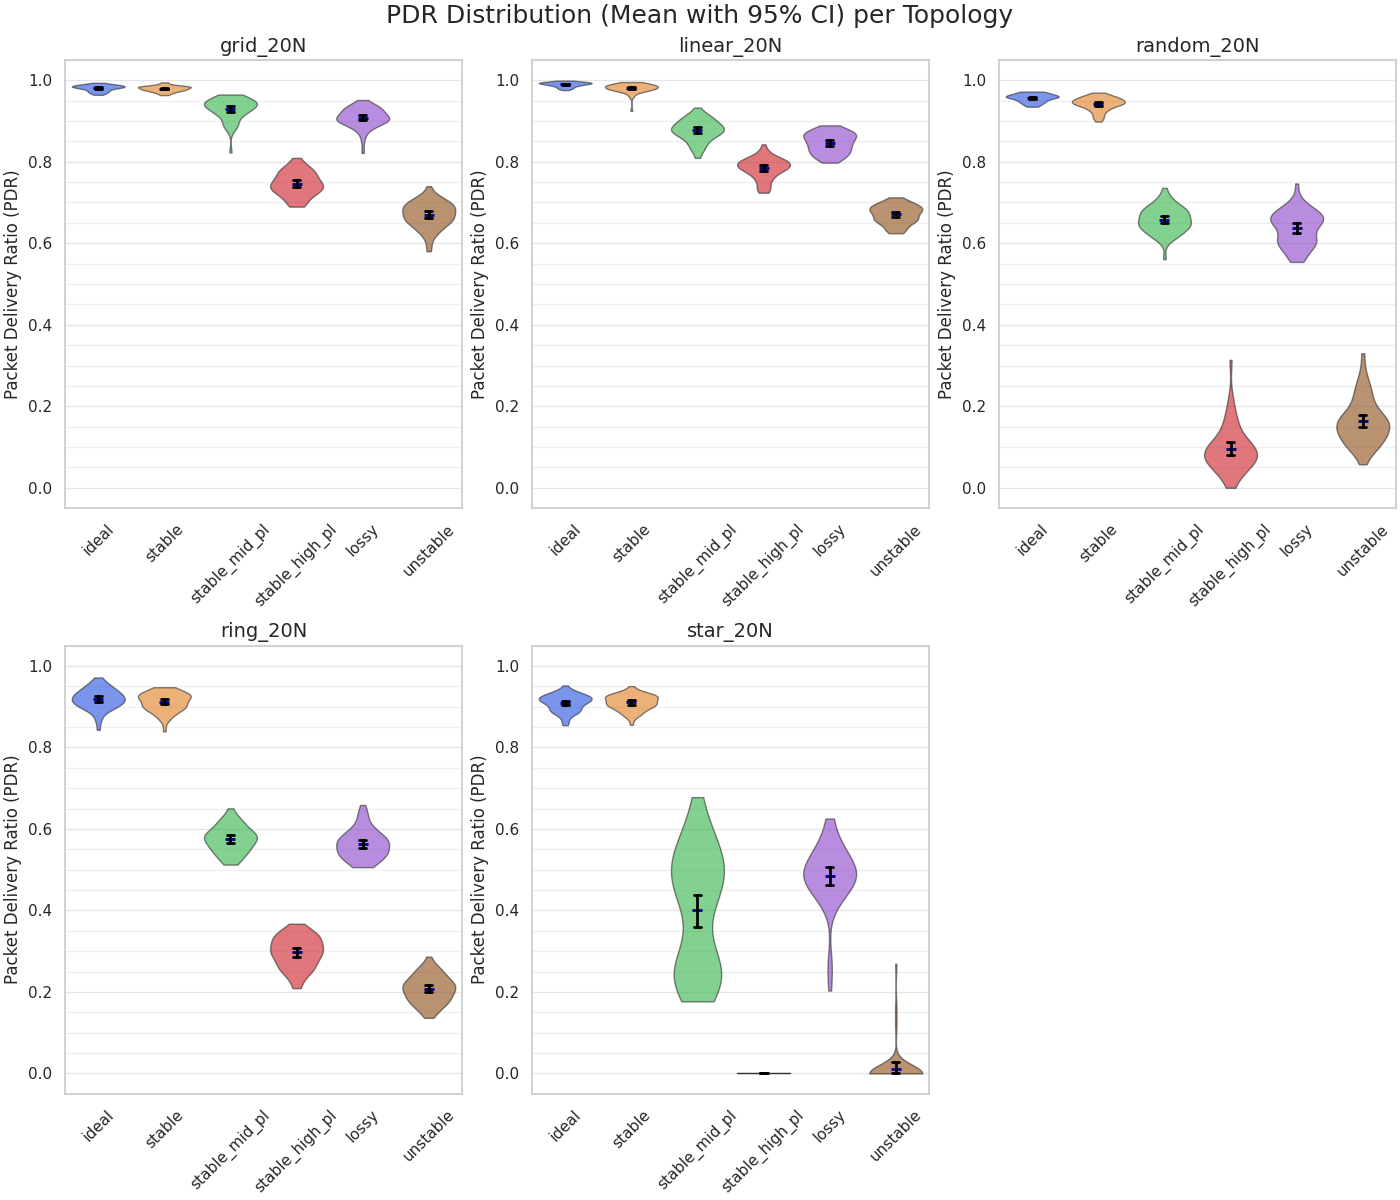
\includegraphics[width=0.8\textwidth]{images/pdr_distribution.png}
\end{frame}

%------------------------------------------------

\begin{frame}{Results: End-to-End Latency}
  \centering
  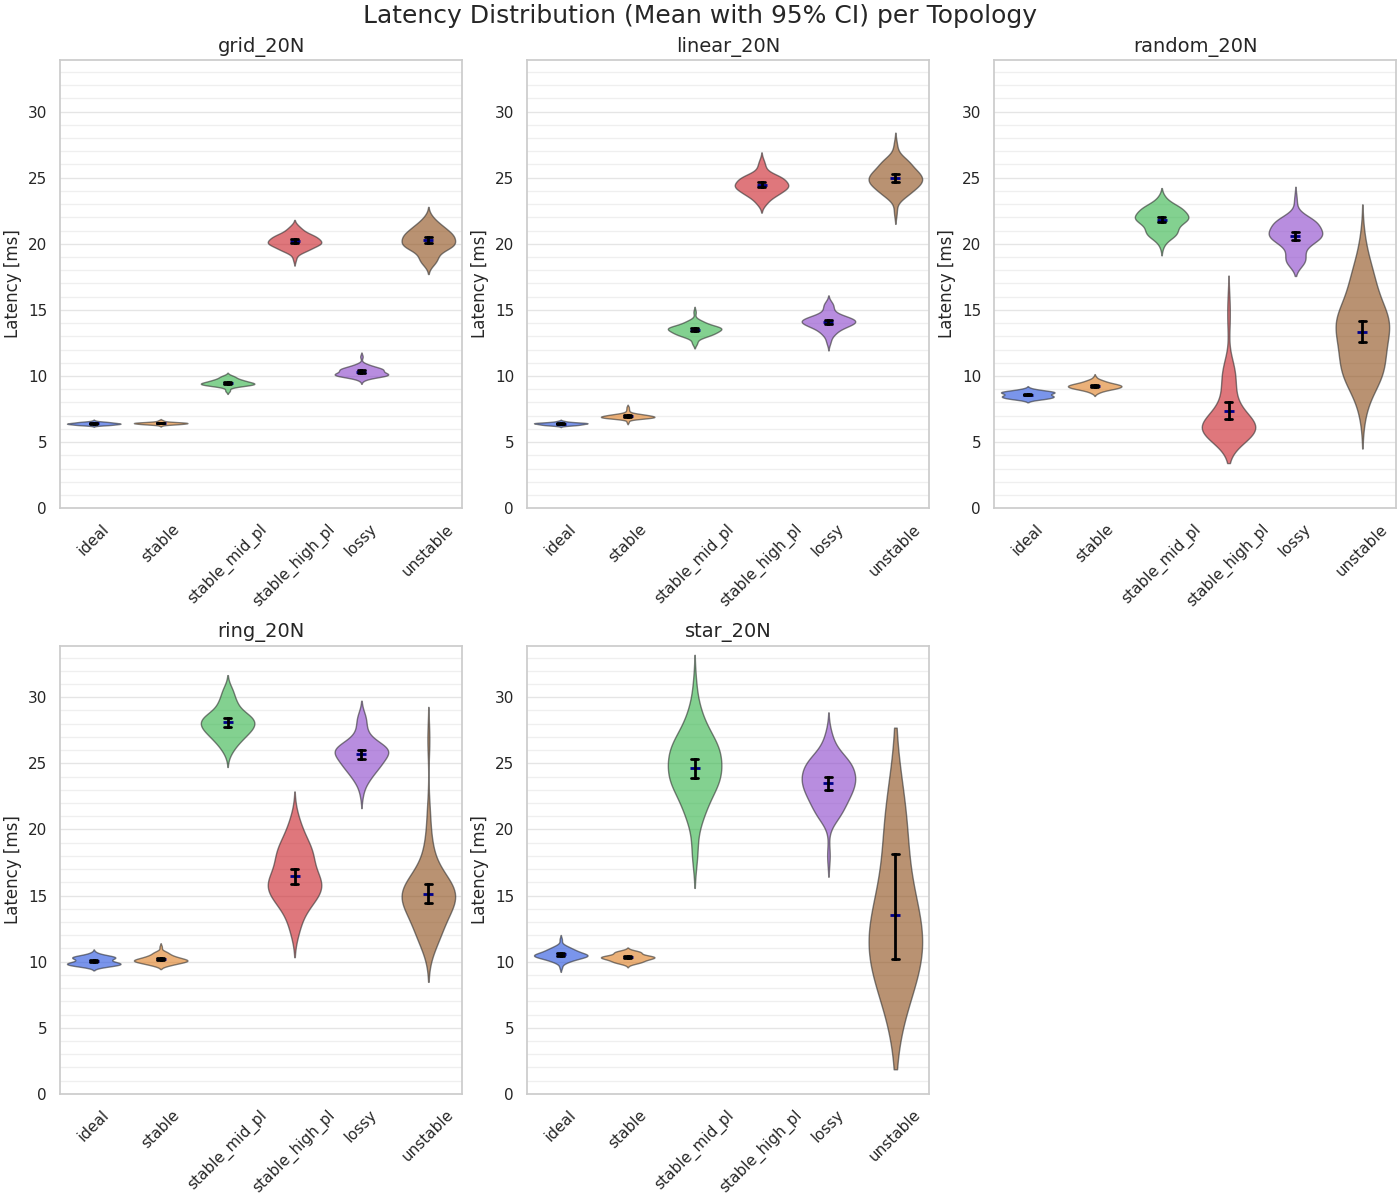
\includegraphics[width=0.8\textwidth]{images/latency_distribution.png}
\end{frame}

%------------------------------------------------

\begin{frame}{Results: Hop Stretch}
  \centering
  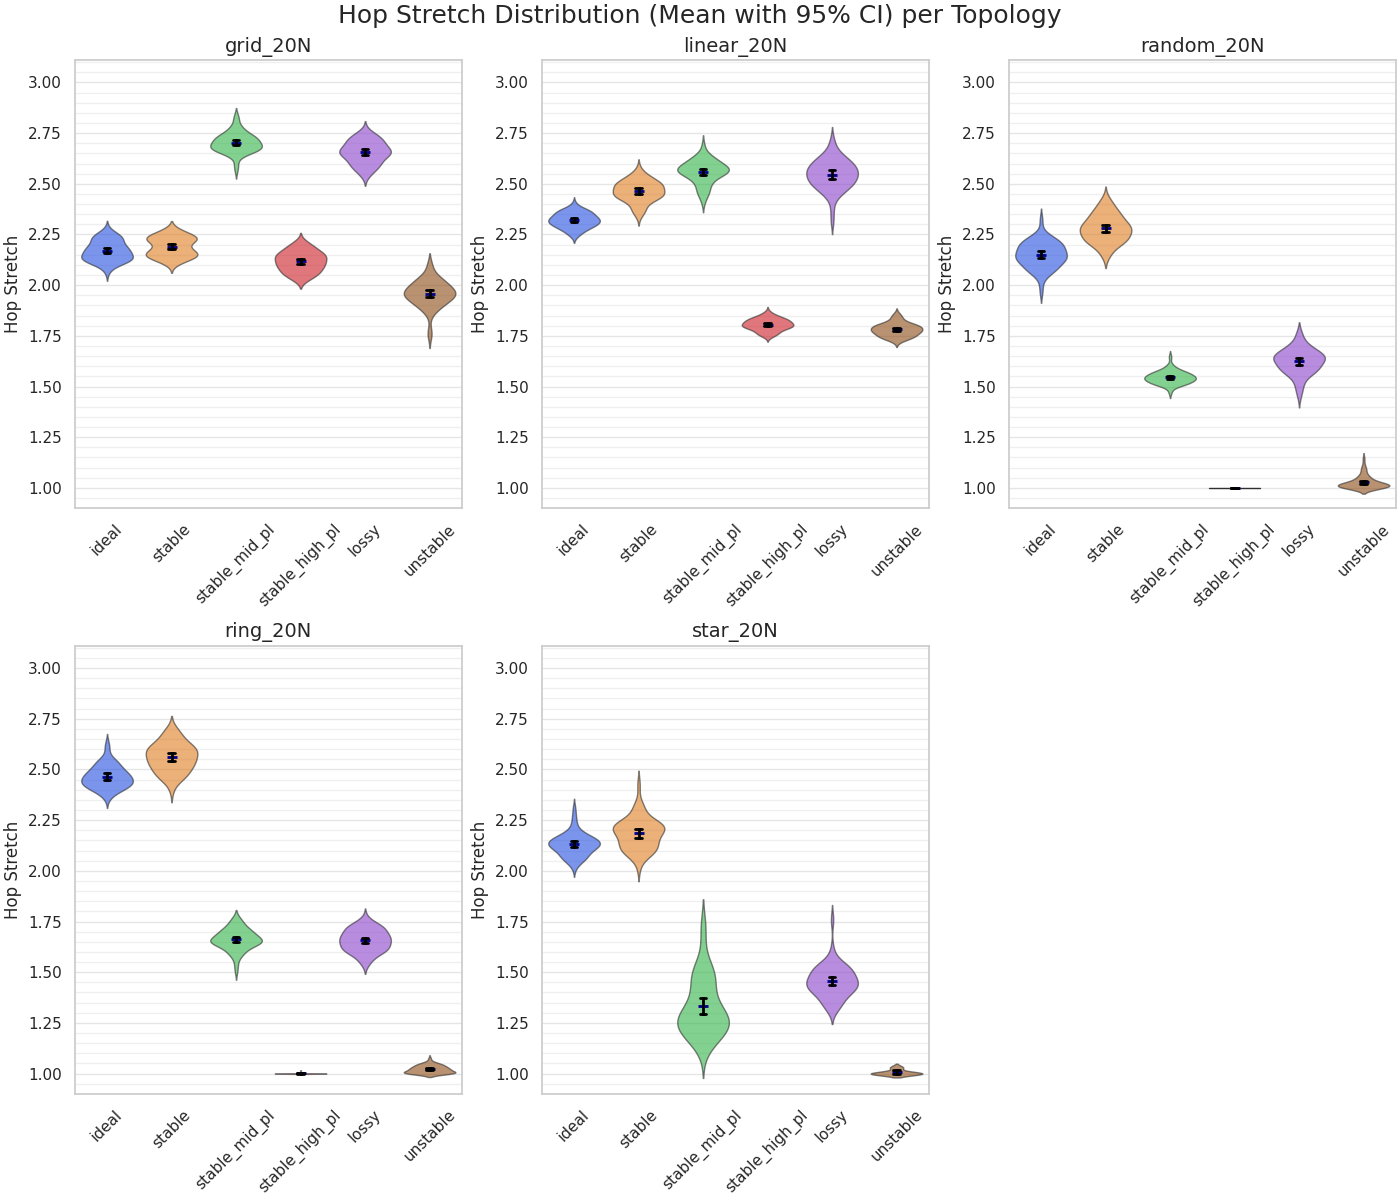
\includegraphics[width=0.8\textwidth]{images/hop_stretch_distribution.png}
\end{frame}

%------------------------------------------------

\begin{frame}{Discussion \& Key Insights}
  \begin{itemize}
    \item Grid and Linear topologies show strongest resilience
    \item Star topology highly sensitive to path loss
    \item Channel instability reduces connectivity
    \item Low hop stretch in severe conditions due to network disconnection
  \end{itemize}
\end{frame}

%------------------------------------------------

\end{document}